%//==============================--@--==============================//%
\subsection[2.5 Socket Programming: Aplicações de Rede]{\hspace*{0.075 em}\raisebox{0.2 em}{$\pmb{\drsh}$} Socket Programming: Aplicações de Rede}
\label{subsec:socket-programming}

Uma aplicação de rede é tipicamente constituída por um par de programas---um programa de \textit{cliente} e um programa de \textit{servidor}---que residem em sistemas terminais distintos. Quando estes programas são executados, é iniciado um \textit{processo de cliente} e um \textit{processo de servidor}, que comunicam entre si ao ler e escrever em \textbf{\textit{sockets}}.

\begin{theo}[\underline{Socket}]{def:socket}\label{def:socket}
    {\footnotesize
        ``A \textbf{network socket} is a software structure within a network node of a computer network that serves as an endpoint for sending and receiving data across the network. The structure and properties of a socket are defined by an application programming interface (API) for the networking architecture. Sockets are created only during the lifetime of a process of an application running in the node. The API for the network protocol stack creates a handle for each socket created by an application, commonly referred to as a \textit{socket descriptor}.''
    }

    \vspace{0.75em}
    \noindent As \textit{sockets} são uma abstração que permite comunicar entre sistemas terminais com o uso de \textit{socket descriptors} standard. Em sistemas UNIX, todas as ações \texttt{I/O} são realizadas ao escrever, e ler, em \textit{file descriptors}.
\end{theo}

%\vspace{-1em}
\begin{figure}[H]
    \centering
    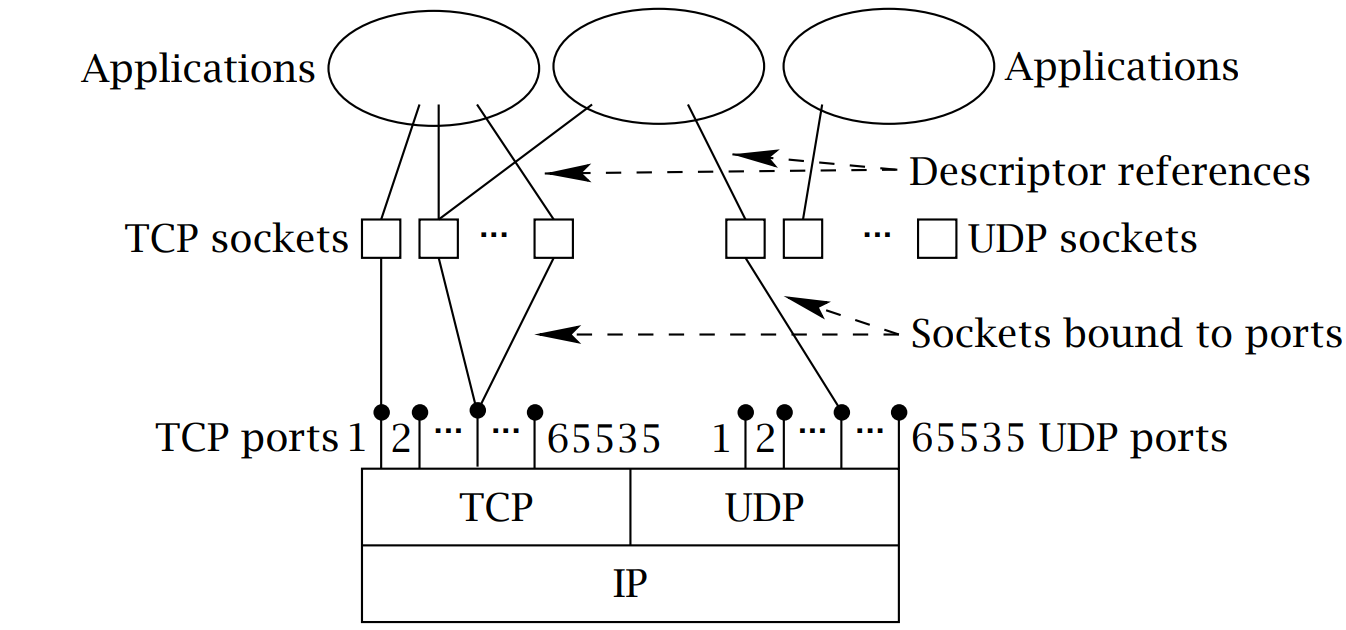
\includegraphics[width = 0.75\linewidth]{img/2/app-sockets-protocols.png}
    \caption{``Logical relationships among applications, socket abstractions, protocols, and port numbers within a single host.''\protect\cite{Donahoo-Kenneth2002}}
    \label{fig:app-sockets-protocols}
\end{figure}

\renewcommand*{\thefootnote}{\fnsymbol{footnote}}
\footnotetext[4]{%
    \textbf{Nota:} Um \textit{file descriptor} (\texttt{fd}) é um inteiro associado a um ficheiro aberto que pode ser: uma conexão de rede, um ficheiro de texto, um terminal...
}
\renewcommand*{\thefootnote}{\arabic{footnote}}

%//==============================--@--==============================//%
\iffalse
\clearpage
\subsubsection[2.5.1]{$\pmb{\rightarrow}$ Socket Programming: UDP}

\begin{lstlisting}[title={UDP\_client.c}]
#include <unistd.h>
#include <stdlib.h>
#include <string.h>
#include <sys/types.h>
#include <sys/socket.h>
#include <netinet/in.h>
#include <arpa/inet.h>
#include <netdb.h>

#define PORT "58001"

int main(void) {
	int fd, errcode;
	ssize_t n;
	socklen_t addrlen;
	struct addrinfo hints, *res;
	struct sockaddr_in addr;
	char buffer[128];

	fd = socket(AF_INET,SOCK_DGRAM,0); //UDP socket
	if (fd == -1) /*error*/ exit(1);

	memset(&hints,0,sizeof(hints));
	hints.ai_family = AF_INET;         //IPv4
	hints.ai_socktype = SOCK_DGRAM;    //UDP socket

	errcode = getaddrinfo("tejo.tecnico.ulisboa.pt",PORT,&hints,&res);
	if (errcode != 0) /*error*/ exit(1);

	n = sendto(fd,"Hello!\n",7,0,res->ai_addr,res->ai_addrlen);
	if (n == -1) /*error*/ exit(1);

	addrlen = sizeof(addr);
	n = recvfrom(fd,buffer,128,0,(struct sockaddr*) &addr, &addrlen);
	if (n == -1) /*error*/ exit(1);
	write(1,"echo: ",6); write(1,buffer,n);

	freeaddrinfo(res);
	close(fd);
}
\end{lstlisting}

%//==============================--@--==============================//%
\subsubsection[2.5.2]{$\pmb{\rightarrow}$ Socket Programming: TCP}

%//==============================--@--==============================//%
\fi